\documentclass{article}


% if you need to pass options to natbib, use, e.g.:
%     \PassOptionsToPackage{numbers, compress}{natbib}
% before loading neurips_2022


% ready for submission
% \usepackage{neurips_2022}


% to compile a preprint version, e.g., for submission to arXiv, add add the
% [preprint] option:
% \usepackage[preprint]{neurips_2022}


% to compile a camera-ready version, add the [final] option, e.g.:
\usepackage{neurips_2022}
\bibliographystyle{plain}

% to avoid loading the natbib package, add option nonatbib:
%    \usepackage[nonatbib]{neurips_2022}


\usepackage[utf8]{inputenc} % allow utf-8 input
\usepackage[T1]{fontenc}    % use 8-bit T1 fonts
\usepackage{hyperref}       % hyperlinks
\usepackage{url}            % simple URL typesetting
\usepackage{booktabs}       % professional-quality tables
\usepackage{amsfonts}       % blackboard math symbols
\usepackage{nicefrac}       % compact symbols for 1/2, etc.
\usepackage{microtype}      % microtypography
\usepackage{xcolor}         % colors
\usepackage{amsmath}
\usepackage{graphicx}
\graphicspath{ {./figures/} }

\newcommand{\vect}[1]{\boldsymbol{#1}}
\newcommand{\mb}[1]{\mathbf{#1}}
\def\RR{\mathbb{R}}
\def\ZZ{\mathbb{Z}}
\def\EE{\mathbb{E}}
\def\PP{\mathbb{P}}
\def\QQ{\mathbb{Q}}
\def\II{\mathbb{I}}
\def\CC{\mathbb{C}}
\def\NN{\mathbb{N}}
\def\OO{\mathbb{O}}
\def\HH{\mathbb{H}}
\def\Ll{\mathcal{L}}
\def\Mm{\mathcal{M}}
\DeclareMathOperator*{\argmin}{arg\,min}


\title{Cross-Dataset Recommender System for \\Overcoming Selection Bias}


% The \author macro works with any number of authors. There are two commands
% used to separate the names and addresses of multiple authors: \And and \AND.
%
% Using \And between authors leaves it to LaTeX to determine where to break the
% lines. Using \AND forces a line break at that point. So, if LaTeX puts 3 of 4
% authors names on the first line, and the last on the second line, try using
% \AND instead of \And before the third author name.


\author{%
  Fengyu Li \\
  Cornell University\\
  \texttt{fl334@cornell.edu} \\
  \And
  Sarah Dean \\
  Cornell University \\
  \texttt{sdean@cornell.edu} \\
}


\begin{document}


\maketitle


\begin{abstract}
  The abstract paragraph should be indented \nicefrac{1}{2}~inch (3~picas) on
  both the left- and right-hand margins. Use 10~point type, with a vertical
  spacing (leading) of 11~points.  The word \textbf{Abstract} must be centered,
  bold, and in point size 12. Two line spaces precede the abstract. The abstract
  must be limited to one paragraph. The abstract paragraph should be indented \nicefrac{1}{2}~inch (3~picas) on
  both the left- and right-hand margins. Use 10~point type, with a vertical
  spacing (leading) of 11~points.  The word \textbf{Abstract} must be centered,
  bold, and in point size 12. Two line spaces precede the abstract. The abstract
  must be limited to one paragraph.
\end{abstract}

\section{Introduction}
Selection bias is one of the most prevalent sources of biases for recommender systems \cite{chen2020bias}. Selection bias happens when there is a pattern in the users' ratings that is unique to the training set. For example, in a recommender system for movies, users might mainly rate movies that are recommended to them, which is a small section of movies already tailored to the users' tastes \cite{pradel2012ranking}. However, the environment the recommender system is deployed on contains all movies regardless of personal tastes. This discrepancy produces a misalignment between training and deployed settings, which is known as a distribution shift. Tackling the selection bias in a recommender dataset has been a constant challenge in designing recommender algorithms\cite{schnabel2016recommendations}.

When recommender systems are deployed in real-world platforms, it is arguably likely that the clients are able to collect rating-associated data from different source distributions. These data (or feedbacks) are either implicit or explicit \cite{aggarwal2016recommender}, while implicit data often comes in a highly-quantized, binary form and explicit data is usually less quantized. For example, a user's explicit rating of a movie is usually quantized to a number between 1 and 5, while the implicit feedback, such as if a user spontaneous searches for a movie, is often binary (more quantized.) We extend our hypothesis and argue that implicit data contains less or no selection bias compared to explicit data. This is because implicit data are often from users' spontaneous actions while explicit data are prejudiced toward the output of the recommender system in the previous feedback loop and also users' innate biases.

In this paper, we attempt to take advantage of datasets from differently quantized sources. More specifically, we proposed a way to feed both a 5-quantized dataset and a binary dataset to any gradient-based recommender algorithm.  To ensure both datasets do not significantly lose their values in the presence of selection bias, we first examine the susceptibility to selection bias of differently quantized datasets from a single distribution. We design experiments under a simulated environment and shows that susceptibility to selection bias is not correlated with the way a dataset is quantized. 

Then, since a less-quantized dataset inherently contains more information than a more-quantized dataset \cite{widrow1996statistical} and thus is more suitable for training, we decided to use it as the training data of matrix factorization and use the more-quantized dataset for propensity scoring and deriving the inverse-probability-scoring (IPS) estimator \cite{thompson2012sampling} \cite{imbens2015causal}, a causal inference approach applicable to matrix completion-based recommender algorithms. In this way, our cross-dataset learning framework empowers existing recommender algorithms to make use of the more quantized, less biased data. We carried out experiment and found our method outperforming baselines by a significant margin.

% Quantization is a practical way to categorize an input from a continuous distribution to a discrete set of bins. We assume the ground truth of a user's rating is a continuous distribution over items because of the inherent impossibility of numerically expressing the feeling of enjoyment and excitement. We treat a recommender dataset as a noised quantization of the ground truth. In other words, users convert their feelings into one of the discrete choices when they rate an item. Recommender datasets are quantized into different degrees. For example, a typical movie rating dataset uses a 5-quantization. A tinder like/dislike dataset uses a 2-quantization.

\section{Related Work}
Prior works on overcoming selection bias-induced distribution shift via a propensity-based approach begins with the seminal paper \cite{schnabel2016recommendations}, which introduces the IPS method into recommender systems. Follow-up works aim at providing a learning-based or behavioral model of user feedbacks for propensity estimation \cite{joachims2017unbiased} \cite{yang2018unbiased}, which remains the central concern of this approach. While many works rely on a propensity matrix that is assumed to be known, TODO our work provides an idea of using a more quantized, implicit dataset for accurate propensity estimation.

The IPS method in our context is, essentially, a method of weighting training examples to correct the bias in the training data. Equivalent approaches such as importance weighting are widely used for domain adaptation in fields other than recommender systems \cite{sugiyama2007covariate} \cite{zhang2018importance}. Discussions on the IPS-based domain adaptation for countering selection bias, which is most relevant to recommender systems, remain limited.

\section{Susceptibility to Selection Bias}
We first examine the susceptibility to selection bias of differently quantized data by manually introducing biased distributions of various degrees to the differently quantized training sets. It is crucial for us that the 2-quantized datasets do not exhibit particular weakness when facing selection bias so that they can be properly adopted for propensity estimation.

\subsection{Simulated Environment for Controlling Bias}
Since selection bias is uncontrollable in a dataset completely drawn from real-world, we have to adopt a simulated environment \cite{krauth2020offline} with both semi-synthetic and synthetic datasets, which shall be explained in section 5. In our environment, we propose the \textbf{softmax observation model} and introduce a hyperparameter $\beta$ to control the degree of bias. For a rating matrix $R$, the corresponding probability matrix of each rating being observed is $\Pr(R_{u,i}\text{ is observed}) = k\text{softmax}(\beta R_{u,i})$, where $k$ is set so that the expected proportion of observed ratings is controlled. The effect of $\beta$ on probability of being observed for different ratings is visualized in figure 1. In our experiment we assume constantly $10\%$ of ratings are observed.
\begin{figure}
  \centering
  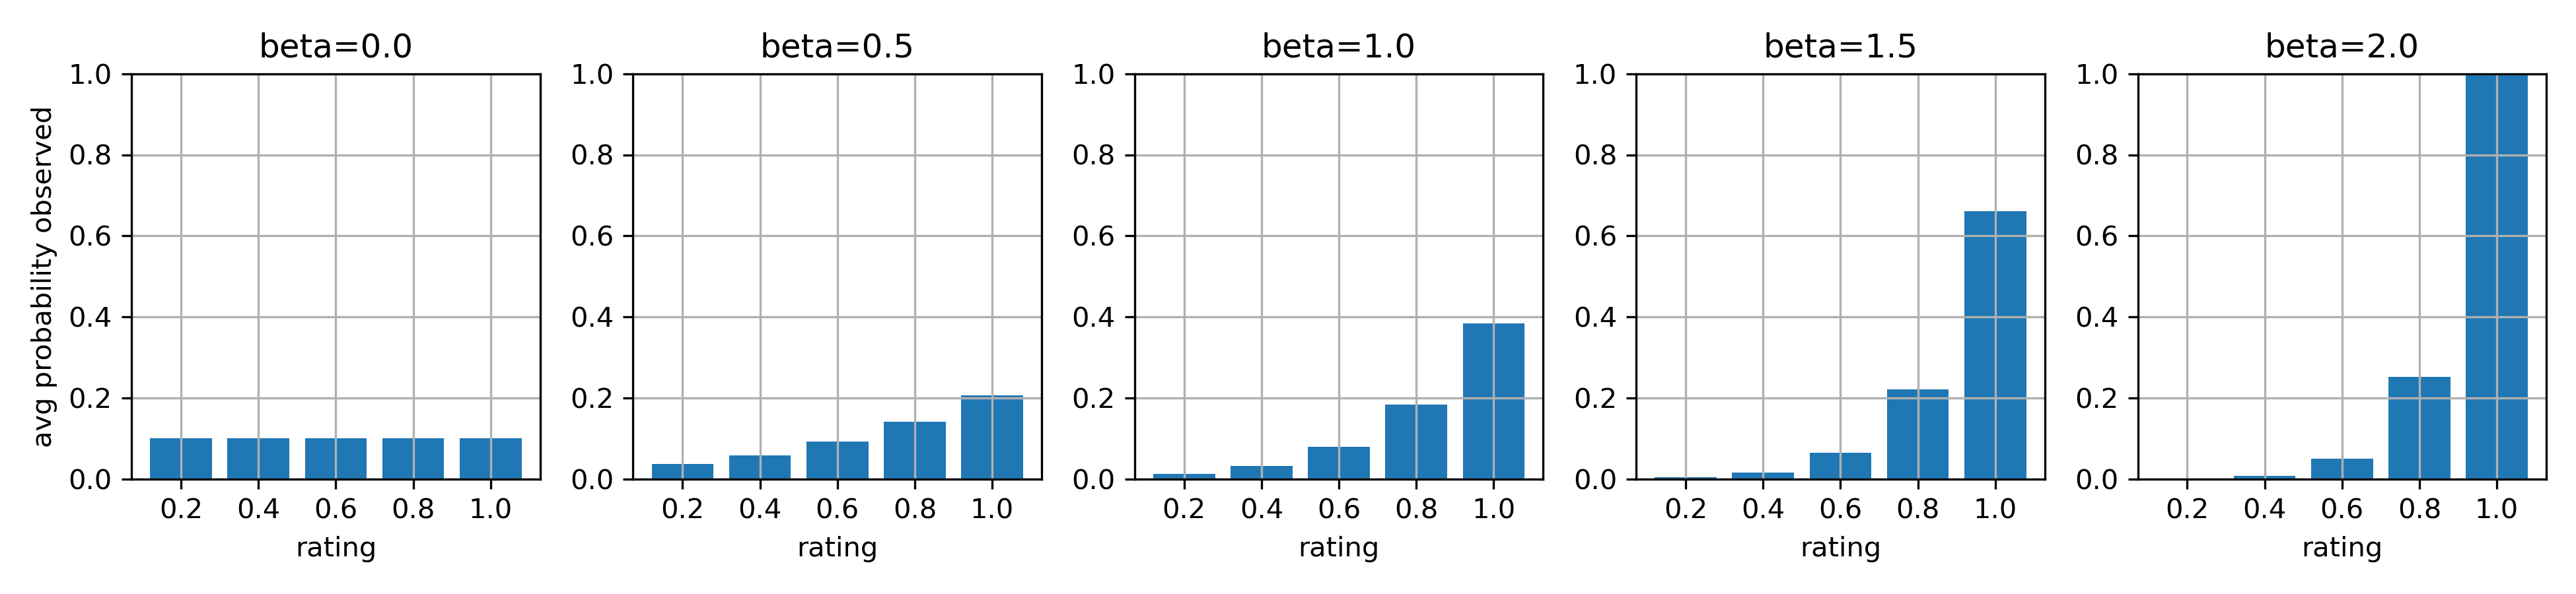
\includegraphics[width=\textwidth]{visualize.png}
  \caption{Visualizing the effect of controlling bias}
\end{figure}

\subsection{Results}
\begin{figure}
  \centering
  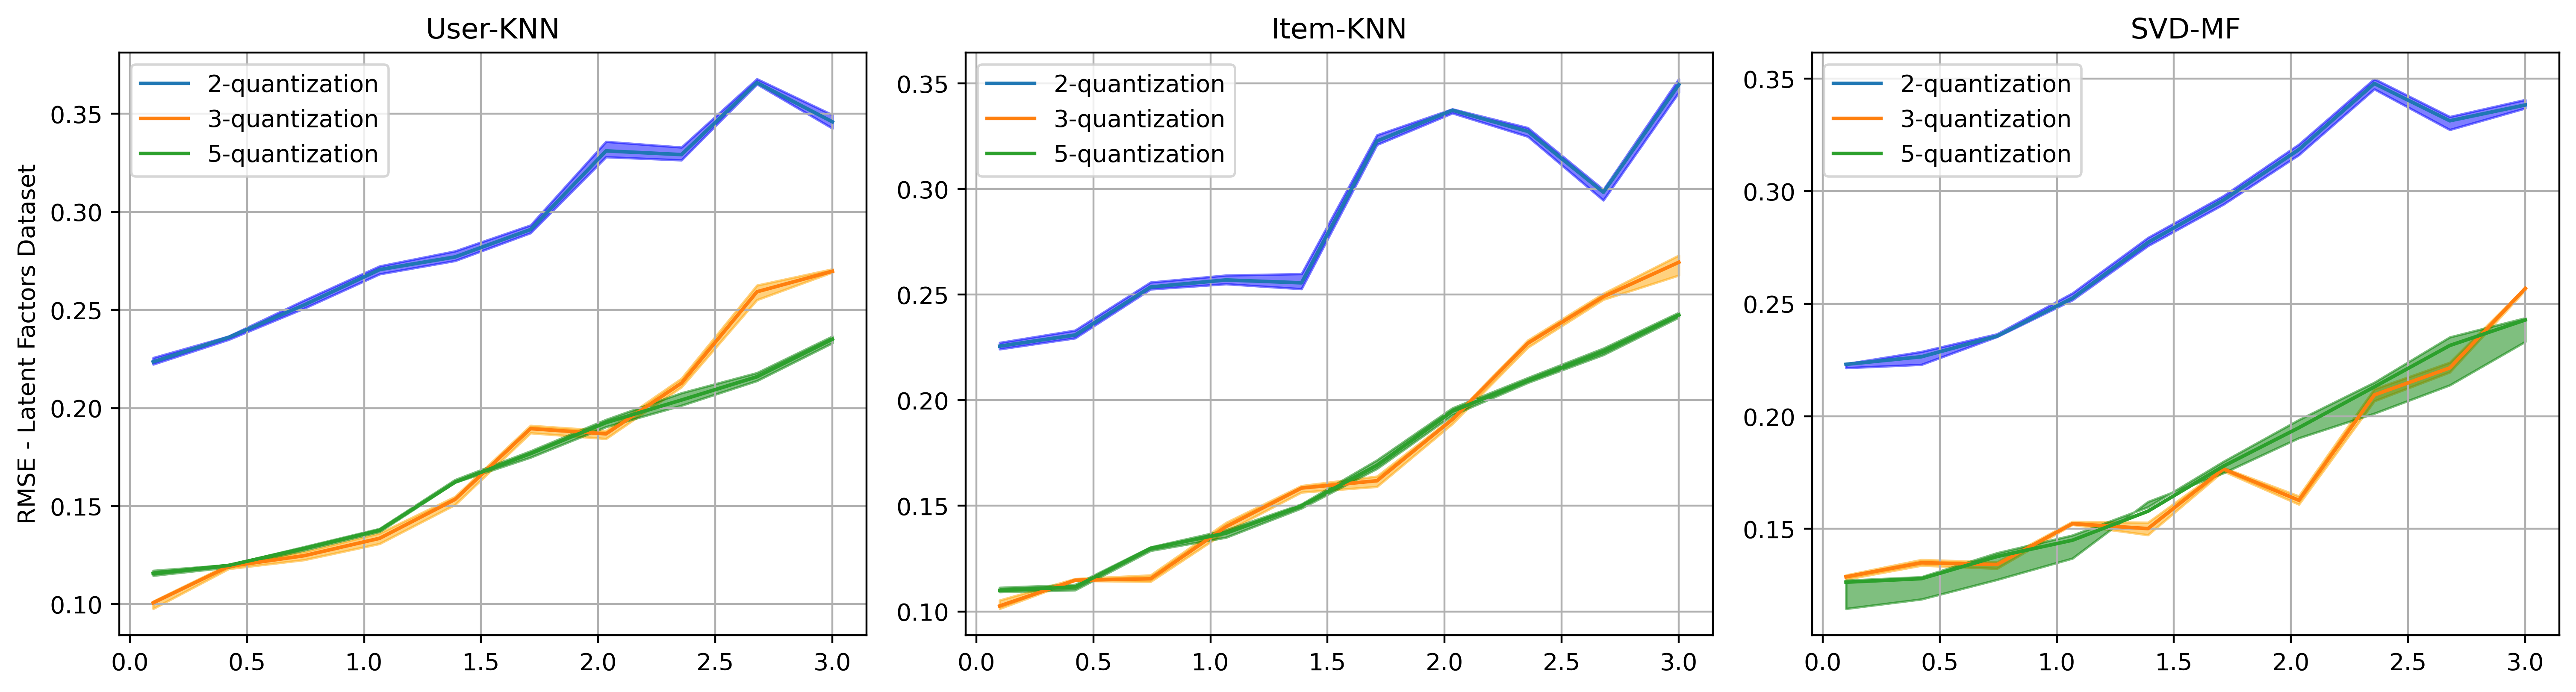
\includegraphics[width=\textwidth]{1.png}
  \caption{The effect of selection bias is not affected by quantization}
\end{figure}
Figure 2 shows our results on two dataset (see section 5) and 3 classic algorithms: user-KNN, item-KNN, and SVD matrix factorization. Although the RMSE grows consistently as $\beta$ increases for all datasets and algorithms, differently quantized datasets do not exhibit significantly different growth rates. We thus conclude it is a viable approach to use the more quantized, less biased dataset for propensity estimation.

\section{Cross-Dataset Propensity Estimation}
With the safety guarantee introduced above, we now turn to our cross-dataset matrix factorization model. Matrix factorization is a simple recommender model that decomposes the rating matrix based on known entries and then predicts the unknown entries\cite{koren2009matrix}. We integrate propensities as \cite{schnabel2016recommendations} did and formulated the recommendation problem as the empirical risk minimization framework below. 
\begin{equation} \argmin_{V,W,A} \frac{1}{N}\left(\frac{(Y_{u,i}- (V_u^TW_i + A))^2}{P_{u,i}} \right) + c \Vert A \Vert^2
\end{equation}
where $A = \{ b_u, b_i, \mu \}$ represents the standard bias parameters (offset), $V$ and $W$ are the decomposed vectors, $\hat{Y} = V_u^TW_i + A$ is the predicted rating, $N$ is the number of ratings, and $c \Vert A \Vert^2$ is the regularizer. The inverse propensity scores $\nicefrac{1}{P_{u,i}}$ are multiplied to each rating during learning, which analogous to re-weighting ratings based on their biases.

Denote the biased training set as $D$. we propose the \textbf{naive-bayes propensity estimator} (NBPE-MF) from a more quantized (binary) dataset $D'$. Essentially,
\begin{equation} 
  P_{u,i} = \Pr(Y_{u,i} \text{ is observed} \mid Y_{u,i} = r_{u,i}) = \frac{\Pr(Y_{u,i} = r_{u,i} \mid Y_{u,i} \text{ is observed})}{\Pr(Y_{u,i}) = r_{u,i}},
\end{equation}
where the numerator can be easily approximated from the dataset, but the denominator requires additional data from less biased sources. In this paper, we estimates the denominator from the unbiased, more quantized dataset using a categorical naive-bayes model. We use $D'$ as a mask to hide biased ratings in the training set from propensity estimation. In other words, $Y_{u,i} \text{ is considered observed}$ only when $D'_{u,i} \text{ is observed}$. 
\begin{equation} 
  NB equation here.
\end{equation}
If the corresponding rating is not captured in $D'$, we set its propensity to the average propensity. 

\section{Experiment}
We designed experiments to verify the performance of our cross-dataset model. We trained on two datasets with $\beta =1$ in training set and used two baseline algorithms for comparison. We selected the root mean square error (RMSE) and the mean absolute error (MAE) as the performance metrics. 

\subsection{Datasets}
\textbf{Imputed ML100K Dataset.}
The ML100K dataset provides 100 thousand MNAR ratings across 1683 movies rated by 944 users and is the standard large-scale dataset used for recommender systems. Since we need the ground truth ratings for controlling bias, we impute the missing ratings using standard matrix factorization. Ratings are normalized between 0 and 1 for consistency with the other dataset. 

\textbf{Latent Factors Simulated Dataset.}
The latent factors dataset is a synthetic dataset that models real-world user behavior. Users and item both have random latent vectors to simulate preferences; both also have biases. The environment is provided by \cite{krauth2020offline}.

\subsection{Baselines}
\textbf{Matrix Factorization (MF.)}
As a simple baseline, we adopt the standard matrix factorization that does not adopt propensity estimation or importance weighting.

\textbf{Naive Propensity Estimator (NPE-MF.)}
The naive propensity estimator naively estimates the propensity scores from the already biased training data and plugs in the results to equation 1.

\textbf{Mixing Datasets Matrix Factorization (MD-MF.)}
To analyze whether our cross-dataset model more efficiently exploits all existing data, we create a larger dataset by mixing the two differently quantized datasets and train the MF algorithm on it.

\subsection{Results}
Table 1 shows the the experiment's results, each entry as the average of five independent trials. Averaged across datasets and metrics, our approach gains 23.1\% reduction in error compared to matrix factorization, 23.1\% compared to naive propensity estimator, and 22.1\% compared to mixing datasets matrix factorization. 

Additionally, we observe that NPE-MF and MF have very similar performance across all settings. This suggests that a IPS-based model will not gain any performance boost if propensities are inaccurately estimated. Furthermore, we argue that our model is data-efficient, i.e., it beats the competitor model (MD-MF), demonstrating that utilizing less biased dataset for propensity estimation is a more viable approach than mixing it with other data, though the latter is sometimes a common engineering practice. On our benchmarks, mixing datasets MF achieves less than 2\% advantage compared to using only one dataset.

We conclude that our cross-dataset model significantly outperforms baselines and provides a efficient way to make use of more quantized (implicit) data. 

\begin{table}0
  \caption{Test set RMSE and MAE for NBPE-MF and baselines}
  \label{sample-table}
  \centering
  \begin{tabular}{lllll}
    \toprule               
                     & \multicolumn{2}{c}{ML100K} & \multicolumn{2}{c}{Latent Factors}                                     \\
    \cmidrule(r){2-5}
                     & RMSE                       & MAE                                & RMSE            & MAE             \\
    \midrule
    MF               & 0.1046                     & 0.0833                             & 0.1331          & 0.1045          \\ 
    NPE-MF           & 0.1048                     & 0.0834                             & 0.132           & 0.1049          \\ 
    MD-MF            & 0.1044                     & 0.083                              & 0.1299          & 0.1027          \\
    \textbf{NBPE-MF} & \textbf{0.076}             & \textbf{0.062}                     & \textbf{0.1065} & \textbf{0.0841} \\ 
    \bottomrule
  \end{tabular}
\end{table}

\section{Conclusion}

\section*{Acknowledgements}

\bibliography{refs}

%%%%%%%%%%%%%%%%%%%%%%%%%%%%%%%%%%%%%%%%%%%%%%%%%%%%%%%%%%%%

\end{document}